\documentclass{classrep}
\usepackage[utf8]{inputenc}
\frenchspacing

\usepackage{graphicx}
\usepackage[usenames,dvipsnames]{color}
\usepackage[hidelinks]{hyperref}
\usepackage{lmodern}
\usepackage{placeins}
\usepackage{url}
\usepackage{amsmath, amssymb, mathtools}
\usepackage{listings}
\usepackage{fancyhdr, lastpage}

\pagestyle{fancyplain}
\fancyhf{}
\renewcommand{\headrulewidth}{0pt}
\cfoot{\thepage\ / \pageref*{LastPage}}

%--------------------------------------------------------------------------------------%
\studycycle{Applied Information Technology, 2 cycle}
\coursesemester{II}

\coursename{Soft Computing Laboratory}
\courseyear{2021/2022}

\courseteacher{dr inż. Kamil Stokfiszewski}
\coursegroup{Wednesday, 8:30}

\author{%
    \studentinfo[239671@edu.p.lodz.pl]{Jan Karwowski}{239671}\\
    \studentinfo[239676@edu.p.lodz.pl]{Kamil Kowalewski}{239676}\\
}

\title{Assignment 2.: MADALINE network for character recognition}

\begin{document}
    \maketitle
    \thispagestyle{fancyplain}

    \tableofcontents
    \newpage

    \section{Main goal}
    \label{main_goal} {
        The main goal of this task is to prepare implementation of MADALINE network.
        MADALINE stands for Multiple Adaptive Linear Elements. The purpose of the
        network is to recognize the single characters with given dimensions (e.g. 4x4).
    }

    \section{Theoretical background}
    \label{theory} {
        MADELINE network is just a series (or a layer) of linear units called
        artificial neurons. Fig. \ref{fig:madeline} presents the structure of such a
        model. It has $M$ inputs, which is propagated to $N$ neurons. Each neuron is
        responsible for identifying single character (e.g. ,,B''). Each neuron has its
        own set of weights, which decides what does it focus on. Value
        of $M$ is determined by image dimension. Respectively value of $N$ is
        determined by number of recognized characters. Normalized value of binarized
        and flattened image template(single for each character) should be used to set
        up neurons' weights values. Given single image template for each character lets
        us easily construct whole MADELINE network.

        \begin{figure}[!htbp]
            \centering
            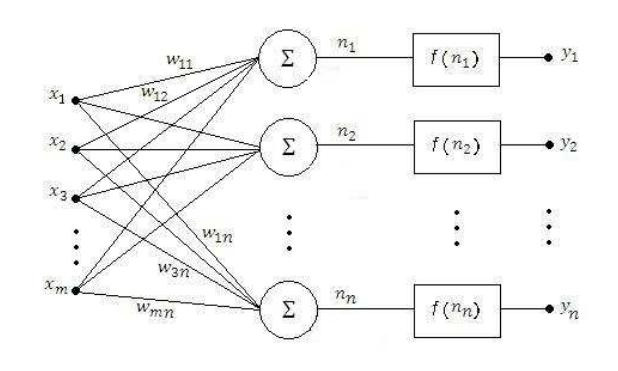
\includegraphics[width=0.8\textwidth]{img/madeline.jpg}
            \caption{Madaline network}
            \label{fig:madeline}
        \end{figure}
        \FloatBarrier
    }

    \section{Implementation details}
    \label{implementation} {
        Program was written in Python programming language and very popular numpy
        library was used as well. The template and test "images" are parsed and loaded
        from txt files. In this approach \textit{#} character is converted to 1 and
        \textit{-} is converted to 0. Thanks to this we can store this artificial image in
        memory of computer and do next computation. The object of Madaline class is
        responsible for accepting the artificial image, which is modeled by in our
        program and return predicted value after calling certain method. The whole
        created infrastructure has been used in main method and results which proves the
        effectiveness of Madaline network are shown after running the program.
    }

    \section{Experiments and results}
    \label{results} {
        In order to explore MADELINE network behaviour simple network was prepared. It
        is created basing on three 4x4 image templates, which describes letters ,,X'',
        ,,Y'' and , ,Z''. These templates are presented in fig.\ref{fig:template_images}.
        To test MADELINE network set of test characters was prepared. It has the same
        structure as template characters, i.e it contains 4x4 images of ,,X'', ,,Y''
        and ,,Z'' letters, but some malformed and negative(inverted) image examples was
        added. These images are presented in fig.\ref{fig:test_images}. After network
        construction all test images were processed by model and results are presented
        in table \ref{tab:results}.

        \begin{figure}[!htbp]
            \centering
            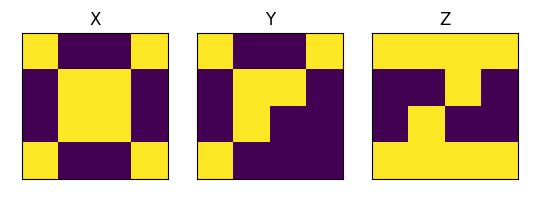
\includegraphics[width=0.8\textwidth]{img/template_images.jpg}
            \caption{Template character images}
            \label{fig:template_images}
        \end{figure}
        \FloatBarrier

        \begin{figure}[!htbp]
            \centering
            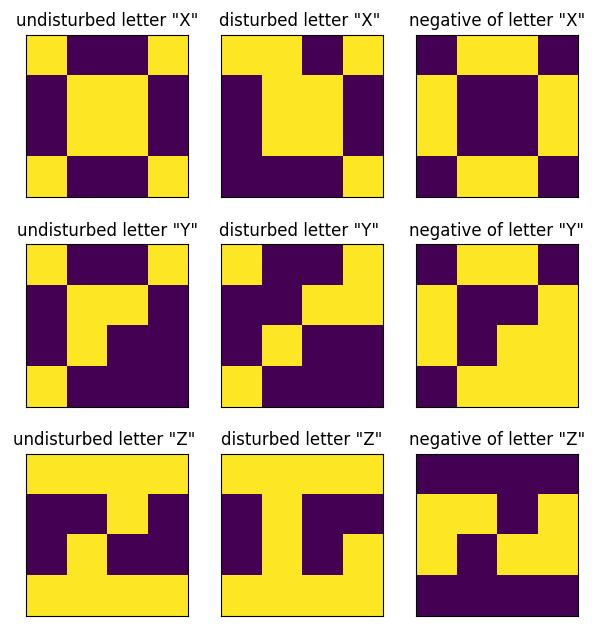
\includegraphics[width=0.8\textwidth]{img/test_images.jpg}
            \caption{Test character images}
            \label{fig:test_images}
        \end{figure}
        \FloatBarrier

        \begin{table}[!htbp]
            \centering
            \begin{tabular}{|l|c|c|c|}
                \hline
                Test pattern name & ,,X'' activation & ,,Y'' activation & ,,Z''
                activation \\ \hline
                undisturbed letter "X" & 1.0 & 0.866 & 0.671 \\
                disturbed letter "X" & 0.875 & 0.722 & 0.671 \\
                negative of letter "X" & 0.0 & 0.0 & 0.447 \\
                undisturbed letter "Y" & 0.866 & 1.0 & 0.645 \\
                disturbed letter "Y" & 0.722 & 0.833 & 0.645 \\
                negative of letter "Y" & 0.224 & 0.0 & 0.5 \\
                undisturbed letter "Z" & 0.671 & 0.645 & 1.0 \\
                disturbed letter "Z" & 0.64 & 0.615 & 0.858 \\
                negative of letter "Z" & 0.289 & 0.167 & 0.0 \\ \hline
            \end{tabular}
            \caption{MADELINE results for test characters set}
            \label{tab:results}
        \end{table}
        \FloatBarrier
    }

    \section{Summary and conclusions}
    \label{summary} {
        Seeing results in table \ref{tab:results} it is simple to find some rule, which
        describes MADELINE behavior. When the network ,,sees'' undisturbed letter, then
        related neuron has possibly high activation ($1.0$). This is the scenario, when
        network can't mistake, because recognized image is exactly same as template
        image - the dot product/correlation reaches its maximum value. Second scenario
        is all about disturbed images. We can say about some sort of lucky, because in
        all the three cases, despite malformed image, proper neuron has the highest
        activation, but there is no such a big difference between $0.875$ and$0.722$ as in
        case of disturbed ,,X''. It is almost sure, that if there were more recognized
        character classes, a pretty small distortion could cause network mistake. Last
        test scenario is very straightforward - undisturbed images were inverted
        producing, ,negatives'' of letters. In such a case proper neuron has exactly
        $0$ activation - there is zero similarity between template image and test image.
    }

    \begin{thebibliography}{0}
        % @formatter:off
        \bibitem{instruction}{Labolatory instruction, URL: https://ftims.edu.p.lodz.pl/pluginfile.php/75438/\\mod\_resource/content/2/soft\_comp\_lab\_02\_MADALINE.pdf}
        % @formatter:on
    \end{thebibliography}

\end{document}
